%% The first command in your LaTeX source must be the \documentclass command.
\documentclass[sigconf,authordraft,anonymous]{acmart}
% \documentclass[manuscript,review,anonymous]{acmart}
%% NOTE that a single column version may required for 
%% submission and peer review. This can be done by changing
%% the \doucmentclass[...]{acmart} in this template to 
%% \documentclass[manuscript,screen]{acmart}
%% 
%% To ensure 100% compatibility, please check the white list of
%% approved LaTeX packages to be used with the Master Article Template at
%% https://www.acm.org/publications/taps/whitelist-of-latex-packages 
%% before creating your document. The white list page provides 
%% information on how to submit additional LaTeX packages for 
%% review and adoption.
%% Fonts used in the template cannot be substituted; margin 
%% adjustments are not allowed.
% added %%%%%%%%%%%%%%%%%%%%%%%%%%%%%%%%%%%%%%%%%%%%%%%% 
\usepackage{booktabs}
% \usepackage{tikz}
% \usetikzlibrary{arrows,shapes, decorations.pathmorphing,backgrounds,positioning}
% \tikzset{every picture/.style={/utils/exec={\sffamily}}}
% \usepackage{subcaption}
\usepackage{subfigure}
\usepackage{amsmath}
\usepackage{multirow}
% added %%%%%%%%%%%%%%%%%%%%%%%%%%%%%%%%%%%%%%%%%%%%%%%% 

%%
%% \BibTeX command to typeset BibTeX logo in the docs
\AtBeginDocument{%
  \providecommand\BibTeX{{%
    \normalfont B\kern-0.5em{\scshape i\kern-0.25em b}\kern-0.8em\TeX}}}

%% Rights management information.  This information is sent to you
%% when you complete the rights form.  These commands have SAMPLE
%% values in them; it is your responsibility as an author to replace
%% the commands and values with those provided to you when you
%% complete the rights form.
\setcopyright{acmcopyright}
\copyrightyear{2018}
\acmYear{2018}
\acmDOI{10.1145/1122445.1122456}

%% These commands are for a PROCEEDINGS abstract or paper.
\acmConference[Woodstock '18]{Woodstock '18: ACM Symposium on Neural
  Gaze Detection}{June 03--05, 2018}{Woodstock, NY}
\acmBooktitle{Woodstock '18: ACM Symposium on Neural Gaze Detection,
  June 03--05, 2018, Woodstock, NY}
\acmPrice{15.00}
\acmISBN{978-1-4503-XXXX-X/18/06}



%%
%% Submission ID.
%% Use this when submitting an article to a sponsored event. You'll
%% receive a unique submission ID from the organizers
%% of the event, and this ID should be used as the parameter to this command.
%%\acmSubmissionID{123-A56-BU3}

%%
%% The majority of ACM publications use numbered citations and
%% references.  The command \citestyle{authoryear} switches to the
%% "author year" style.
%%
%% If you are preparing content for an event
%% sponsored by ACM SIGGRAPH, you must use the "author year" style of
%% citations and references.
%% Uncommenting
%% the next command will enable that style.
%%\citestyle{acmauthoryear}

%%
%% end of the preamble, start of the body of the document source.
\begin{document}

%%
%% The "title" command has an optional parameter,
%% allowing the author to define a "short title" to be used in page headers.
\title[Multi-level Context for Informational Bias Detection by Contrastive Learning and GAT]{Modeling Multi-level Context for Informational Bias Detection by 
Contrastive Learning and Sentential Graph Network}

%%
%% The "author" command and its associated commands are used to define
%% the authors and their affiliations.
%% Of note is the shared affiliation of the first two authors, and the
%% "authornote" and "authornotemark" commands
%% used to denote shared contribution to the research.

% \author{Shijia Guo}
% \affiliation{%
%   \institution{Shanghai Jiao Tong University}
%   \streetaddress{800 Dongchuan Rd.}
%   \city{Shanghai}
%   \country{China}
%   \postcode{200240}}
% \email{seveny1997@sjtu.edu.cn}

% \author{Kenny Q. Zhu}
% \affiliation{%
%   \institution{Shanghai Jiao Tong University}
%   \streetaddress{800 Dongchuan Rd.}
%   \city{Shanghai}
%   \country{China}
%   \postcode{200240}}
% \email{kzhu@cs.sjtu.edu.cn}


%%
%% By default, the full list of authors will be used in the page
%% headers. Often, this list is too long, and will overlap
%% other information printed in the page headers. This command allows
%% the author to define a more concise list
%% of authors' names for this purpose.
% \renewcommand{\shortauthors}{Trovato and Tobin, et al.}

%%
%% The abstract is a short summary of the work to be presented in the
%% article.
\begin{abstract}
Informational bias is widely present in news articles. 
It refers to providing one-sided, selective or suggestive information of specific aspects of certain entity to guide a specific interpretation, thereby biasing the reader's opinion. Sentence-level informational bias detection is a very challenging task in a way that such bias can only be revealed together with the context, examples include collecting information from various sources or analyzing the entire article in combination with the background. In this paper, we integrate three levels of context to detect the sentence-level informational bias in English news articles: adjacent sentences, whole article, and articles from other news outlets describing the same event. Our model, MultiCTX (Multi-level ConTeXt), uses contrastive learning and sentence graphs together with Graph Attention Network (GAT) to encode these three degrees of context at different stages by tactically composing contrastive triplets and constructing sentence graphs within events. Our experiments proved that contrastive learning together with sentence graphs effectively incorporates context in varying degrees and significantly outperforms the current SOTA model sentence-wise in informational bias detection.
\end{abstract}

%%
%% The code below is generated by the tool at http://dl.acm.org/ccs.cfm.
%% Please copy and paste the code instead of the example below.
%%
% \begin{CCSXML}
% <ccs2012>
%  <concept>
%   <concept_id>10010520.10010553.10010562</concept_id>
%   <concept_desc>Computer systems organization~Embedded systems</concept_desc>
%   <concept_significance>500</concept_significance>
%  </concept>
%  <concept>
%   <concept_id>10010520.10010575.10010755</concept_id>
%   <concept_desc>Computer systems organization~Redundancy</concept_desc>
%   <concept_significance>300</concept_significance>
%  </concept>
%  <concept>
%   <concept_id>10010520.10010553.10010554</concept_id>
%   <concept_desc>Computer systems organization~Robotics</concept_desc>
%   <concept_significance>100</concept_significance>
%  </concept>
%  <concept>
%   <concept_id>10003033.10003083.10003095</concept_id>
%   <concept_desc>Networks~Network reliability</concept_desc>
%   <concept_significance>100</concept_significance>
%  </concept>
% </ccs2012>


%   \begin{CCSXML}
%     <ccs2012>
%       <concept>
%           <concept_id>10002951.10003317.10003318</concept_id>
%           <concept_desc>Information systems~Document representation</concept_desc>
%           <concept_significance>500</concept_significance>
%           </concept>
%       <concept>
%           <concept_id>10010405.10010455.10010461</concept_id>
%           <concept_desc>Applied computing~Sociology</concept_desc>
%           <concept_significance>500</concept_significance>
%           </concept>
%       <concept>
%           <concept_id>10003033.10003034.10003035</concept_id>
%           <concept_desc>Networks~Network design principles</concept_desc>
%           <concept_significance>300</concept_significance>
%           </concept>
%      </ccs2012>
%     \end{CCSXML}
    
\ccsdesc[500]{Information systems~Document representation}
\ccsdesc[500]{Applied computing~Sociology}
\ccsdesc[300]{Networks~Network design principles}
  
  


%%
%% Keywords. The author(s) should pick words that accurately describe
%% the work being presented. Separate the keywords with commas.
\keywords{bias detection, informational bias, media bias, news bias, graph neural networks, contrastive learning, contextual modeling
}

%% A "teaser" image appears between the author and affiliation
%% information and the body of the document, and typically spans the
%% page.
% \begin{teaserfigure}
%   \includegraphics[width=\textwidth]{sampleteaser}
%   \caption{Seattle Mariners at Spring Training, 2010.}
%   \Description{Enjoying the baseball game from the third-base
%   seats. Ichiro Suzuki preparing to bat.}
%   \label{fig:teaser}
% \end{teaserfigure}

%%
%% This command processes the author and affiliation and title
%% information and builds the first part of the formatted document.
\maketitle

\section{Introduction}

Protein$-$protein interactions (PPIs) are of central importance for the majority of biological functions, such as signal transduction, metabolic pathways, molecular dynamics, and protein networks\cite{Hoffmann.Krallinger.ea:2005}, for they serve as the most fundamental building blocks of the entire interacademic systems of any organisms. Collecting data on pairwise interaction relationships is essential for multiple purpose, including identification of modules with certain functionality\cite{Spirin.Mirny.03}, mapping diseases to dominated genes\cite{Ideker.Sharan.08}, and after all, understanding wholistic metabolic/genetic networks from a system biology perspective.

A lot of databases have been built to store protein and genetic interactions from major model organism species and are available in various standardized formats, such as MINT\cite{Zanzoni.Montecchi-Palazzi.ea:2002}, BIND\cite{Bader.ea:2003}, BIOGRID\cite{DBLP:journals/nar/StarkBRBBT06}, etc. Among those mainstream databases, the data largely rely on voluntary reports by scientists or researchers, besides, comprehensive curation efforts become indispensable for the sake of accuracy. However, the amount of biology-related literatures with respect to protein interactions grows explosively and thus make it either impossible or impractical to manually detect PPI information anymore.

Considering huge amount of PPI information with great wealth hidden in published papers, in recent years, numerous mining techniques have been proposed that aim to extract PPI information automatically from free text, especially machine learning, information retrieval, and natural language processing\cite{DBLP:journals/bib/WinnenburgWPDS08}.These approaches can be roughly categorized into three classes: co$-$occurrence, rule$-$based, and machine learning. 

Co$-$occurrence is the approach with most simplicity and naivete. Just as its name implies, this method intends to find out pairs of proteins that co-occur in the same context. The scope of "same context" ranges from phrase, sentence, paragraph to whole abstract, even document. The underlying assumption is that whenever two proteins are mentioned together by authors, chances are high that there is some kind of relationship between them. However, however, in-context closeness even semantic relation does not necessarily represent actual biological interaction. As a consequence, a large fraction of candidate pairs are mismatched inevitably, causing a high recall but low precision.

The second approach is rule-based extraction, in other words, pattern matching. There are many types of rules, most of them concern natural language processing (NLP). One way is to specify hand-crafted regular expressions before hand, which mostly lean on language usage preference. Besides, by using full or partial (shallow) parsing strategies, more information would be acquired, such as part-of-speech taggers, local dependencies between syntactic components, context-free grammar\cite{DBLP:journals/bioinformatics/TemkinG03}, and full sentence structure. Compared to co$-$occurrence, rule-based approach enjoy better precision but much lower recall. In addition, since the rules are usually derived from training data, that is to say, the improper choice of training data would be significantly lethal, therefore quality of extraction is invariably instable and may not applicable to other data.

The third and most commonly used approach use machine learning techniques, in this case, the task to extract protein$-$protein interactions turns out to be a binary classification problem. Each protein pairs are represented along with a set of features, which is associated with their context, then a well$-$defined classifier gives the answer whether the candidate protein pairs is classified to be qualified PPI. (TO BE FURTHER FILLED!!!)

In this paper, we introduce a general bootstrapping framework for Protein$-$protein interaction extraction from natural text.Our method differs from most of the previous works in three aspects:

(1)The extraction process is driven by only tiny fraction of training data, which are regarded as seed data. In each round, it would derive reliable patterns automatically from seed data, then extract more positive PPI pairs consequently, what's more, the seed data would be augmented by the newly extracted results with high confidence.

(2)multiple graph kernel. 

(3)various evaluation.




% \input{chap/2-Data}
\section{Approach}
%We first present our methods for testing short circuits in
%models, then modify some of these methods to create
%training data to reverse the short circuit problem
%and enhance the robustness of the models.
% 
%\subsection{Proxy Test for Short Circuit}
%We propose two types of approaches that can be used as proxy test for short circuits.
%One is through inspecting attention maps in
%the models under a white-box setting.
%The other is to generate new test cases by applying different operations on correct choices under a black-box setting.
%
%
%\subsubsection*{White-box Attention Weights~(AW)}
%One intuitive way to detect if an attention-based model is 
%exploiting short circuits is to visualize its attention map. 
%Given a well-trained model and a correctly answered MCQ  in the 
%form of \textit{[CLS] premise [SEP] choice [SEP]}, 
%where \textit{[CLS]} and \textit{[SEP]} are model-dependent 
%delimiters and \textit{choice} refers to the correct choice, 
%we first tokenize the input, feed the token sequence into the model, 
%and extract the attention map of all attention heads from the 
%last encoder layer.
%
%The attention maps are visualized through off-the-shelf tool~\cite{vig-2019-multiscale}
%into user-friendly demo as shown in \figref{fig:att-goodex}. 
%Human annotators are then asked to determine whether there exists 
%strong attention connections from the correct choice to the premise. 
%We consider the MCQ is solved without short-circuiting only if 
%over half of the annotators label it as having strong attention 
%connections. 
%
%Though accurate, such manual annotation is cost-prohibitive to be 
%scaled to larger tests. To remedy this issue, we propose 
%a rule-based procedure to automatically detect the short circuit 
%behavior of a model on MCQ. Specifically, we aggregate the 
%attention maps into one individual map by max-pooling over all 
%attention heads. Then we check if there exists at least one 
%attention score between token in the choice and token in the premise 
%higher than threshold $t_1$ or at least two higher than threshold 
%$t_2$, excluding special tokens like comma and period. 
%We consider that the model not short-circuiting on this MCQ if 
%neither of the two conditions is met. In practice, the 
%threshold $t_1$ and $t_2$ are tuned so as to maximally simulate 
%human annotation. The pseudo-code is shown in Algorithm \ref{AW}.
%
In this section, we first present our methods for testing short circuits in models, and then modify some of these methods to create training data to address the short circuit problem and enhance model robustness.

\subsection{Proxy Test for Short Circuit}
Since no existing method can definitively prove if a model is short-circuiting on a question, we propose two types of approaches that serve as proxy tests for short circuits. These approaches reveal the effects of model short-circuiting, though they can't directly prove the short-circuit itself, similar to dark matter. One approach involves inspecting attention maps in models under a white-box setting, while the other generates new test cases by applying different operations on correct choices under a black-box setting.

\subsubsection*{White-box Attention Weights~(AW)}

One intuitive way to detect if an attention-based model is exploiting short circuits is to visualize its attention map. Given a well-trained model and a correctly answered MCQ in the form of \textit{[CLS] premise [SEP] choice [SEP]}, where \textit{[CLS]} and \textit{[SEP]} are model-dependent delimiters and \textit{choice} refers to the correct choice, we first tokenize the input, feed the token sequence into the model, and extract the attention map of all attention heads from the last encoder layer.

The attention maps are visualized through an off-the-shelf tool~\cite{vig-2019-multiscale} into a user-friendly demo, as shown in \figref{fig:att-goodex}. Human annotators are then asked to determine whether there exists strong attention connections from the correct choice to the premise. We consider the MCQ to be solved without short-circuiting only if over half of the annotators label it as having strong attention connections.

Although accurate, such manual annotation is cost-prohibitive to be scaled to larger tests. To remedy this issue, we propose a rule-based procedure to automatically detect the short circuit behavior of a model on MCQ. Specifically, we aggregate the attention maps into one individual map by max-pooling over all attention heads. Then we check if there exists at least one attention score between a token in the choice and a token in the premise higher than threshold $t_1$, or at least two higher than threshold $t_2$, excluding special tokens like comma and period. We consider the model to not be short-circuiting on this MCQ if neither of the two conditions is met. In practice, the thresholds $t_1$ and $t_2$ are tuned to maximally simulate human annotation. The pseudo-code is shown in Algorithm \ref{AW}.


\begin{algorithm}
\small
	\caption{Attention Weight Thresholding}
	\label{AW}
\hspace*{0.02in} {\bf Input:} 
premise $P$, correct choice $C$, model $M$,  threshold $t_1$ and $t_2$. \\
\hspace*{0.02in} {\bf Output:}
binary 0/1 label $L$.
	\begin{algorithmic}[1]
		\State initialize counters $c_1$ and $c_2$ to 0.
		\State tokenize the formatted input as sequence of tokens $S$.
		\State feed $S$ into $M$ and extract the last layer's attention maps $Attn_{all}$.
		\State aggregate $Attn_{all}$ into $Attn_{max}$ by max-pooling over all attention heads.
		\For{$w_1$ in $C$}
		\For{$w_2$ in $P$}
		\If{$Attn_{max}(w_1, w_2)> t_1$}
				$c_1$ += 1
		\EndIf
		\If{$Attn_{max}(w_1, w_2) > t_2$}
				$c_2$ += 1
		\EndIf
		\EndFor
		\EndFor
		\State output 1 if $c_1>0$ or $c_2\geq 2$ and 0 otherwise.
	\end{algorithmic}
\end{algorithm}

\subsubsection*{Black-box Choice Operator}
\label{sec:proxy}
While attention-based testing methods can detect short circuits within the encoder directly, they don't directly detect short circuits in the end-to-end MCQ model, which also includes a linear layer above the attention-based pretrained language model. Additionally, these methods are limited to a family of models with inherent attention mechanisms.

A more desirable approach is an automatic end-to-end black-box test that is model-independent. In black-box testing, if a model correctly answers an MCQ, we slightly modify the MCQ by applying a certain``operation'' on the original correct choice to produce another wrong choice. The newly generated MCQ must share the same correct choice as the original question. By observing the model's response to the second MCQ, we can infer whether the model short-circuits on the original MCQ.If the model still selects the correct choice, then we consider it to have passed the test and not short-circuited on the original MCQ. The challenge now is how to construct the new wrong choice by implementing the operation in various ways.

In this paper, we consider the operations listed in \tabref{table:proxyop}. Some of the operations were mentioned in previous literature, while others are proposed here (marked with *).
The first line in each cell describes the operation, and the next two lines provide an example of constructing a false choice from a choice in the original question. An operation may either preserve (p) the truth value (\crosssymbol $\rightarrow$ \crosssymbol) or change (c) the truth value of the choice (\checksymbol $\rightarrow$ \crosssymbol).

\begin{table}[th]
        \centering
        \scriptsize
        \begin{tabular}{l|l}
                \toprule
                \textbf{Oper.} &\textbf{Description and Example}\\
                \hline
                \multirow{3}{*}{Neg+} & Add negation (c) \\
                & \textit{They called the police to come to my house. \checksymbol} \\
                & \textit{They {\color{olive}{didn't}}  called the police to come to my house. \crosssymbol} \\
                \hline
                \multirow{3}{*}{Neg-} &Remove negation (c) \\
                & \textit{Ben {\color{olive} never} starts working out. \checksymbol} \\
                & \textit{Ben starts working out. \crosssymbol}\\
                \hline

                \multirow{3}{*}{NER} &Randomly replace person names (c)\\
                 & \textit{A big wave knocked {\color{olive} Mary} down . \checksymbol} \\
                & \textit{A big wave knocked {\color{olive} Kia} down . \crosssymbol} \\
                \hline
                \multirow{3}{*}{PR*} & Switch pronoun by gender or quantity (c)\\
        &\textit{{\color{olive} She} had a great time .\checksymbol} \\
        &\textit{{\color{olive} He} had a great time . \crosssymbol} \\
                \hline
                \multirow{3}{*}{PI*} &Instantiate pronoun by randome person (c) \\
        &\textit{{\color{olive} They} gave Tom a new latte with less ice . \checksymbol}\\
        &\textit{{\color{olive} Nathanael} gave Tom a new latte with less ice . \crosssymbol}\\
                \bottomrule
%               \hline
                \multirow{3}{*}{Adv} &Add adverbs for emphasis (c) \\
                &\textit{The ocean was a calm as a bathtub .\crosssymbol} \\
                &\textit{{\color{olive} In fact} the ocean was a calm as a bathtub .\crosssymbol} \\
                \hline
               \multirow{3}{*}{CO*} & Crossover: Swap the true choices between two questions (p)\\ 
	&\textit{\color{olive}Josh got sick . \checksymbol} \\
	&\textit{\color{olive}{She had a great time .\crosssymbol}}  \\
\hline
                \multirow{3}{*}{Syn} &Replace adj/adv with synonym (p) \\
                &\textit{Dawn felt {\color{olive} happy} about getting away with it . \crosssymbol} \\
                &\textit{Dawn felt {\color{olive} glad} about getting away with it . \crosssymbol} \\

		\bottomrule
               \multirow{3}{*}{MT*} & Mutate: Swap two consecutive words (c) \\
		& \textit{Deb said yes {\color{olive} to} {\color{olive} Tim} 's marriage proposal. \crosssymbol} \\
		& \textit{Deb said yes {\color{olive} Tim} {\color{olive} to} 's marriage proposal .\crosssymbol} \\
               \hline
\multirow{3}{*}{Voice} &Swap subject and object (c) \\
        & \textit{{\color{olive}{Kara}} asked {\color{olive}{the neighbors}}  not to litter in their yard . \checksymbol} \\
        &\textit{{\color{olive}{the neighbors}} asked  {\color{olive}{Kara}}  not to litter in their yard . \crosssymbol}\\
                \bottomrule
        \end{tabular}
        \caption{A number of operations considered for proxy testing. 
First line in each cell describes the operation, the next two lines
give an example of how to construct a false choice from a choice of
the original question. An operation may either 
preserve (p) the truth value (\checksymbol $\rightarrow$ \checksymbol, \crosssymbol $\rightarrow$ \crosssymbol) or change (c) the truth value of
the choice (\checksymbol $\rightarrow$ \crosssymbol).  }
        \label{table:proxyop}
\end{table}

Inspired by boundary testing in software engineering, we can classify these operations into three equivalent classes (three vertical sections in \tabref{table:proxyop}), depending on the nature of the \textit{false} choice constructed:
\begin{enumerate}
\item The syntax and semantics are correct, and the \textit{false} choice appears similar to the \textit{true} choice.
\item The syntax and semantics are correct, and the \textit{false} choice appears distinct from the \textit{true} choice.
\item Either syntax or semantics is incorrect.
\end{enumerate}

The last class is not suitable for testing short circuits because the model may answer the proxy question correctly by eliminating the false choice due to errors in it, not by considering the premise.

We focus on perturbations on negation~\cite{checklist2020acl}, NER~\cite{checklist2020acl}, and pronouns in the first class and adverbial~\cite{wsp2020acl}, crossover, and synonym~\cite{checklist2020acl,wsp2020acl} in the second class.

While most of the operations are self-explanatory, the \textit{crossover} operation is unique and deserves special attention. Inspired by molecular biology, for each MCQ in the dataset that the model answers correctly, we substitute the original false choice with the true choice from another randomly sampled MCQ. The substituted choice remains false in the proxy question. The operation can be visually explained in \figref{fig:cross}.

\begin{figure}[th]
\centering
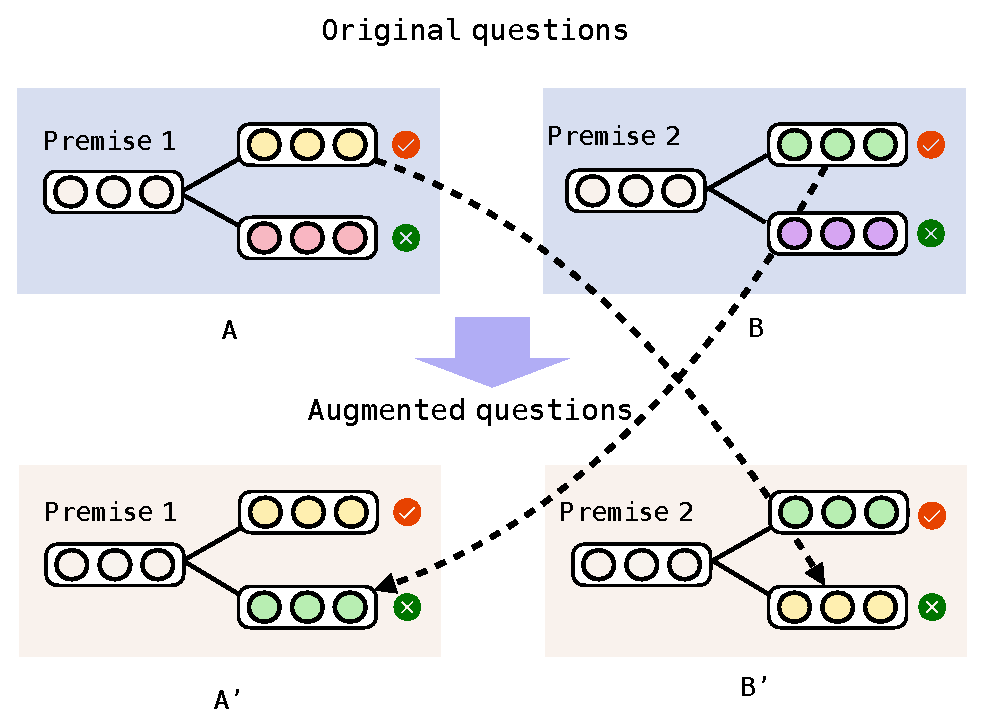
\includegraphics[width=\columnwidth]{figure/cross.eps}
\caption{The Crossover Operation: the true choice of both questions
are used to replace the false choices of these questions to create
two new proxy questions.}
\label{fig:cross}
\end{figure}

Compared to all other operations in classes 1 and 2, the crossover provides a proxy question that is most different from the original one but easier from a human perspective. This is because the two choices may be quite unrelated. If the model does not handle it correctly, it may be more indicative of a short circuit. As a result, the crossover is potentially a better short circuit test than others.

Another advantage of the crossover operation is that we can generate multiple false choices for an original question at a low cost, allowing us to test each original question more thoroughly. In contrast, most other operations cannot produce an adequate number of different variants of the original choice.

In summary, the proposed black-box choice operator provides a more generalizable and model-independent method for detecting short circuits in MCQ models. By applying various operations to create proxy questions, we can assess the model's performance and robustness more accurately, contributing to the development of better and more reliable models in the future.

\subsection{Improving Model Robustness by Data Augmentation}

If a model is shown to short-circuit by the proxy tests, its performance may decline, especially when applied to out-of-domain test data. To make models more robust, one natural thought is to generate more data to encourage models to focus on the relation between the premise and choices. While the operations used to generate proxy tests can also be utilized for data augmentation, not all of them are scalable or able to generate enough data for training.

The two operations that can generate a substantial amount of data are crossover and mutation. These operations can be applied to the training data to enhance the model's robustness.

\subsubsection*{Crossover for Data Augmentation}

Crossover is a good option for data augmentation because the two choices were originally true answers in their respective questions and presumably carry spurious features if the model was short-circuiting. By incorporating crossover into the training data, the model is forced to consider the premise in order to determine which choice is better.

\subsubsection*{Mutation for Data Augmentation}

Mutation has two flavors: (1) swap the words only in the true choice; (2) swap the words both in the true and the false choice. Compared to crossover, mutation has the potential to be more effective at improving model robustness. It not only forces the model to look into the premise due to its two very similar choices (same set of tokens), but also makes the model more sensitive to fine differences in word orders and enhances the model's prior grammatical knowledge.

\subsubsection*{Differentiating between Proxy Test and Data Augmentation}

It is essential to differentiate between the use of crossover and mutation operations in proxy tests and data augmentation. In proxy tests, these operations are used to modify the test data to assess the model's short-circuiting behavior. In contrast, when applied for data augmentation, the same operations work on the training data to enhance the model's robustness and generalization capabilities.

In conclusion, data augmentation through crossover and mutation operations can contribute to improving model robustness by encouraging models to focus on the relationship between the premise and choices. By incorporating these operations into the training data, models are forced to consider the premise and become more sensitive to the fine differences in word orders, leading to better performance and reliability in real-world applications.

\section{Experiments}
\label{sec:experiments}
In this section, we conduct
extensive experiments on slogan generation 
to evaluate the performance
of the proposed model SALE.
We introduce the dataset, 
the competing models and parameter settings,
as well as the evaluation metrics.
We also demonstrate the experimental results in a series of evaluations
and perform further analyses on the effectiveness of our approach
in generating accurate, fluent, informative and attractive slogans.

\subsection{Dataset}
\label{sec:dataset}
We first introduce the text corpora we create
for slogan generation task in e-commerce.
Then we describe the evaluation dataset we used in
our following experiments.
The datasets are released at \url{https://202.120.38.146/slogan/}.

\subsubsection{Dataset for Slogan Generation}
\label{sec:corpora}
%In this section, we describe the experimental setup,
%especially the hyper-parameter configurations of 
%the Seq2Seq framework we used in following experiments. 
%We also detail dataset used in our experiments.
Slogan generation in E-commerce is a relative new problem.
Thus, there is a lack of dataset for this task.
We created a new dataset, containing 
the basic information of the topics attending to potential focuses or selling-points,
including the topic and its item preference, as well as the slogan.
The data are collected from Taobao, a large-scale website for e-commerce in China.

We use the pattern of ``\emph{PV} + \emph{CG}" 
to construct topics from frequent phrases mining from largely amount
of query logs and product titles.
The product titles are composed by the sellers and content producers on the
website.
We construct multiple item preferences for each topic by sampling items from 
secondary categories as well as human intervention to 
make the items with an item preference concentrate more on a specific focus 
or selling-point.
Thus, in each instance, a topic is annotated with an item preference semi-automatically
by leveraging the category ontology introduced in \secref{sec:introduction}.
Then, we recruit experts to write a slogan for each data instance.
Overall, the dataset contains 857 topics and 
in total 3,555 $(x, p, y)$ instances after preprocessing.

We use four splits named (train/dev/LMdev/test) in our experiments.
Note that, the LMdev split is for 
hyper-parameter $\beta$ tuning (see \secref{sec:shallow_fusion} in details).
The splits are randomly divided based on topics 
proportionally by 90\%, 5\%, 1.5\% and 3.5\%.
Thus each split of (train/dev/LMdev/test) includes 771, 43, 13, 30 topics separately,
and correspond to 3132 training instances, 231 development instances, 
50 LM development instances, as well as 142 test instances.

%For the evaluation dataset, 
\subsubsection{Evaluation Dataset}
\label{sec:eval_dataset}
We perform algorithm evaluation and human evaluation
in our experiments (see \secref{sec:metrics} in details).
Thus we provide two evaluation datasets separately for each.
We directly use all the 142 instances of test split in \secref{sec:corpora},
referred as FULLtest,
for the algorithm evaluation which are based on automatic scoring systems,
such as BLEU.
Besides, we randomly sample 50 instances from the test split
to form a small evaluation dataset for human evaluation,
referred as HUMtest.


\subsection{Compared Methods}
\label{sec:compared}
In this section, we introduce the baseline and choices for 
our model components, as well as the parameter settings
used in those models.

\subsubsection{Baselines and SALE}
\label{sec:baselines}
According to the problem statement (in \secref{sec:problem})
and the proposed item preference fusion methods (in \secref{sec:preference}),
the models for comparison backed by Seq2Seq framework are mainly one-way input models and two-way input models.

One-way input models (prefixed by \emph{One}) takes in one-way input as the source sequence,
and the slogan as its target sequence, without considering 
semantics enhancement or incorporating pretrained language model.
There are three one-way input baselines with different inputs.
\textbf{One-T} (\textbf{t}opic) model
takes the topic itself as its source sequence,
while \textbf{One-P} (item \textbf{p}reference) model takes
the titles of items as its source sequence.
Then, 
%while 
\textbf{One-CAT} (con\textbf{cat}nating) model 
concatenates the topic and its item preference with special token \emph{SEP}
as a separator, and takes the sequence of concatenation as its source sequence.

The two-way input models (prefixed by \emph{Two})
are designed to treat topics and item preferences heterogeneously.
We propose two kinds of two-way input models
based on different heterogeneous inputs fusion methods 
(see details in~\secref{sec:preference}).
%we propose two fusion methods in \secref{sec:preference}
%to combine the heterogeneous inputs.
\textbf{Two-BiAttn} (\textbf{bi}directional \textbf{att}ending) model use the two-way bidirectional attending
to combine the representations of topics and that of item preferences.
\textbf{Two-CAT} (con\textbf{cat}nating) model use two-way concatenating strategy 
to fuse the heterogeneous outputs of encoders.

For \textbf{SALE}, 
we incorporate the semantics enhancement module
(in \secref{sec:semantics}) to enrich
the deep contextualized representations
backed by Two-CAT baseline.
\textbf{SALE+PLM} integrates
%On the basis of SALE, 
%we integrate
pre-trained language model (PLM) 
into SALE at inference time in order to improve
the generalization and robustness of the model.
%Specially, SALE identifies the \emph{is-a} relations
%among heterogeneous inputs and
%increase the semantic capacity of the model for better contextualized representations
%knowledge-aware module

\subsubsection{Parameter Settings}
We use an architecture of 8 stacked convolutional layers 
for both the topic encoder and the item preference encoder
as well as the decoder parts with kernel width as 3.
To enable deep convolutional networks, 
we add residual connections~\cite{he2016deep} from the input of each convolution
to the output of the layer as well.
For each convolutional layer, we set the hidden vector size as 512
and the embedding size as 256.
To alleviate the overfitting problem, we add the dropout ($p=0.2$)
layer~\cite{srivastava2014dropout} for all convolutional layers and fully connected layers.

To optimize the proposed models,
we use Nesterov's accelerated gradient method
~\cite{sutskever2013importance} with gradient clipping 0.1
~\cite{pascanu2013difficulty},
momentum 0.99, and 
learning rate 0.2.
We terminate the training process when the learning rate drops 
below 10e-5.
We set beam size as 5 for the beam search algorithm
in the testing step.
The hyper-parameter $\beta$ of SALE-PLM (in ~\eqnref{eq:shallow_fusion})
was selected to maximize the generation performance
on the LMdev split by grid search, from the range 1e-4 and 0.1.


\subsection{Evaluation Metrics}
\label{sec:metrics}
We perform both algorithm evaluation and human evaluation
in our experiments.
Specially, we evaluate our model on generation quality which includes
the automatic scoring metrics such as
BLEU and lexical diversity,
as well as a number of human-evaluation metrics.

\paragraph{BLEU}
The BLEU algorithm~\cite{papineni2002bleu} compares consecutive phrases of the 
generated slogan with the consecutive phrases it finds
in the reference slogan, and counts the number of matches, in a weighted fashion.
A higher BLEU score indicates a higher degree of similarity with the reference
slogan.
We compare all competing models on test split in terms of the BLEU score as a sanity check.
We also use BLEU score as the standard metric to finetune
hyper-parameter $\beta$ in SALE+PLM model.

\paragraph{Lexical Diversity}
A common problem in automatic text generation is that the system tends to generate safe
answers with enough diversity~\cite{li2016deep}.
A low diversity score often means generated contents are general and vague, 
while higher diversity means the generated contents are more informative and 
interesting.
Following~\cite{ChenLZYZ019}, we calculate the number of distinct n-grams produced on the test split
as the measurement of the diversity of generated descriptions.

\paragraph{Human-evaluation Metrics}
Automatic scoring metrics including BLEU score and lexical diversity are competitive and inexpensive to operate.
However, they do not consider
other important aspects such as intelligibility and grammatical correctness (or fluency) of slogan.
We use several human-evaluation metrics
to evaluate competing models on various perspectives.
\begin{itemize}
	\item \textbf{Overall quality} is designed to measure the
	overall generation quality of model.
	\item \textbf{Relevancy} is used to measure the content relevancy of generated slogan to the given topic and items.
	\item \textbf{Fluency} focus on the intelligibility and grammatical correctness of generated slogan.
	\item \textbf{Interestingness} takes personification and attractiveness into account.
\end{itemize}


\subsection{Performance Comparisons and Analysis}
\label{sec:results}


In this section, we conduct an analysis of our proposed model
to evaluate the contribution of item preference fusion module and
semantics enhancement module as well as the integration of 
pre-trained language model.

We evaluate competing models on FULLtest and HUMtest 
as we described in \secref{sec:eval_dataset}.
The comparison results of slogan generation are shown in 
\tabref{tab:auto_eval} and \tabref{tab:human_eval}.
For human evaluation, we recruit three experts as annotators 
and ask them to give scores on each aspect of generated slogan, 
range from 1 to 5,
then average the scores of each aspect on HUMtest as 
human evaluation results.


\begin{table*}[th]
	%	\small
	\centering
	\caption{Slogan generation results comparison with baseline methods using FULLtest.}
	\label{tab:auto_eval}
	\begin{tabular}{lcccc}
		\hline
		Model %& Overall quality 
		& BLEU &  Diversity (n=2) ($\times 10^2$ )& Diversity (n=3) ($\times 10^2$ ) & Diversity (n=4) ($\times 10^2$ ) \\
		\hline
		One-T %&  3.30  
		&  28.34 &  2.25   &  2.45  &  2.37 \\
		One-P %&  3.86  
		&  41.11 &   4.74 &    5.99 & 6.33 \\
		One-CAT  % & 3.82  
		& 38.86  &  3.86 &  4.77  & 4.94 \\
		Two-BiAttn  % & 3.86  
		& 36.99  &  4.82 &  5.87  &  6.03   \\
		Two-CAT % & 3.95
		& 40.59  &  4.89 &  5.99  &  6.22 \\
		\hline\hline
		SALE % & \textbf{4.16}  
		& 42.31  & 4.87  &  6.20 &  6.55  \\
		SALE+PLM % & -  
		& \textbf{42.36}   &  \textbf{4.89} & \textbf{6.23}  &  \textbf{6.57}  \\
		%		SingleSG$_{\mathrm{concept}}$ & 28.34 &  3.30 & 3.32 & 4.31 & 4.38 \\
		%		SingleSG$_{\mathrm{items}}$& 41.11 & 3.84 & 4.0 & 4.30 & 4.22  \\
		%		MultiSG-{biattn} & 36.99 & 3.86 & 4.05 & 4.17 & 4.11 \\
		%		MultiSG-{cat} & 40.59 & 3.95 & 4.13 & 4.34 & 4.23  \\
		\hline 
	\end{tabular}
\end{table*}



\begin{table}[th]
	\small
	\centering
	\caption{Human evaluation for slogan generation task using HUMtest.}
	\label{tab:human_eval}
	\begin{tabular}{lcccc}
		\hline
		Model & Overall quality & Relevancy &  Fluency & Interestingness \\
		\hline
		One-T &  3.30  &  3.32 &  4.31   &  4.38 \\
		One-P &  3.84 &  4.0 &   4.30 &    4.22  \\
		One-CAT  &  3.62  & 3.94  & 4.24  & 4.18  \\
		Two-BiAttn  & 3.86  & 4.05  &  4.16  &  4.11     \\
		Two-CAT & 3.95  & 4.13  &  4.34 &  4.23   \\
		\hline\hline
		SALE & \textbf{4.16}  & \textbf{4.32}  & \textbf{4.53}  &  \textbf{4.43}  \\
		SALE+PLM & -  & -   &  - &   -  \\
		%		SingleSG$_{\mathrm{concept}}$ & 28.34 &  3.30 & 3.32 & 4.31 & 4.38 \\
		%		SingleSG$_{\mathrm{items}}$& 41.11 & 3.84 & 4.0 & 4.30 & 4.22  \\
		%		MultiSG-{biattn} & 36.99 & 3.86 & 4.05 & 4.17 & 4.11 \\
		%		MultiSG-{cat} & 40.59 & 3.95 & 4.13 & 4.34 & 4.23  \\
		\hline 
	\end{tabular}
\end{table}



Firstly, we show the importance of item preference for  slogan generation.
We introduce item preference features for specific topic
using category ontology as discussed in \secref{sec:preference}.
Topic and its item reference are simply concatenate into one input sequence
in One-CAT model. 
As we can see that One-CAT substantially outperforms One-T which only use topic as input
with an advantage of +0.32 overall quality (relatively 9.7\%), +10.5 BLEU, +110.7\% diversity ($n=2$), +144\% diversity ($n=3$) and +81\% diversity ($n=4$),
Thus, item preference plays an important role in slogan generation task.

However, the results show that
One-P model which only takes in item preference as input outperforms
One-CAT on various metrics.
This imposes that topic and item preference are two heterogeneous inputs,
thus we should treat them differently in the model using item preference fusion method.
Next, we analyze the contribution of item preference fusion methods proposed
in \secref{sec:preference}
by comparing One-CAT, Two-BiAttn and Two-CAT.
We can see that show that two-way concatenating method for Two-CAT
substantially outperforms two-way directional attending for Two-BiAttn.
Though Two-CAT model slightly decreases on BLEU compared to One-P,
Two-CAT outperforms One-P according to human evaluation shown in \tabref{tab:human_eval}.
This suggests that two-way bidirectional attending fusion 
makes the semantics corruption between two heterogeneously deep contextualized representations.
Therefore, two-way concatenating fusion method is more effective for 
heterogeneous inputs combination.

Our proposed \emph{is-a} knowledge-aware model SALE 
is backed by Two-CAT, equipping with the semantics enhancement module.
Results show the effectiveness of semantics enhancement module
proposed in \secref{sec:semantics}.
As shown in \tabref{tab:human_eval} and \tabref{tab:auto_eval}, 
SALE outperforms Two-CAT by a substantial margin.
Specially, semantics enhancement improves the
diversity scores ($n=3, 4$) 3.5\%, 5.3\% separately .
SALE also achieves an improvement of 1.72 (relatively 4.24\%) in terms of BLEU, 
as well as an improvement of 0.57 in terms of overall quality.
We can see that SALE outperforms all previous baselines on every aspect.
Thus SALE is able to generate accurate, fluency, informative and attractive slogans.
We further illustrate this in \secref{sec:cases}. 



Lastly, we analyze the contribution of pre-trained language model integration
comparing results of SALE and SALE+PLM.
As shown in \tabref{tab:auto_eval}, 
incorporating PLM at inference stably improves the diversity 
that performs best at every n-gram diversity scores ($n=2,3,4$).
Note that, we finetuned hyper-parameter $\beta$ for SALE+PLM 
in terms of BLEU score on LMdev split,
and SALE+PLM with $\beta = 2e\mathrm{-}4$ achieves best BLEU score as 42.94.
Thus, we use $\beta=2e\mathrm{-}4$ for SALE+PLM model in test.
As shown in \tabref{tab:auto_eval}, SALE+PLM 
outperforms all competing models in terms of BLEU score as 42.36 
on FULLtest dataset.
Since the results generated by SALE and SALE+PLM are nearly the same on HUMtest,
their human evaluation results are same, 
we do not show result of SALE+PLM in \tabref{tab:human_eval}.
We can see that in this case the improvement of PLM integration is minor but stable, 
on both BLEU score and diversity scores.
We argue that such PLM integration makes our model more robust.

% the contribution of item preferences in one-way input models: OneT, OneP, OneCAT
% item preference fusion methods for two-way input models: OneCAT, Two-BiAttn, Two-CAT
% is-a knowledge-aware model SALE: Two-CAT, SALE, SALE+PLM




\subsection{Case Studies}
\label{sec:cases}
In this section, we perform case studies to observe 
how our propose methods influence the generation so that
the model can generate different slogans for a specific topic
according to different item preferences.
Besides, our proposed \emph{is-a} knowledge-aware model SALE generate higher quality slogans
benefiting from semantics enhancement.

%The running example in \tabref{sec:introduction} illustrates 

In \tabref{tab:vary_preference}, % \tabref{tab:vary_preference}
two item preferences are provided for topic ``早教玩具" (early education toys).
The first preference consists of musical toys such as ``音乐拍拍鼓" (musical patting drum),
which focuses on music education for children,
while the second preference is mainly about ``手摇铃" (rattle) which focuses on improving concentration ability 
as well as soothe emotions for babies.
The second example of 
\tabref{tab:vary_preference} is the running example we discussed in \secref{sec:introduction}.
The proposed model SALE successfully captures those focuses 
and generate attractive slogans accordingly.
For example, SALE generates \emph{music enlightenment}
for the focus of musical patting drum
and generates \emph{soothe baby's emotion } for the focus of 
rattle.
As shown in \tabref{tab:vary_preference}, 
we use red color to mark the preferences and its effects for slogan generation.

We also demonstrate the effectiveness of semantics enhancement
by comparing slogans generated by SALE and Two-CAT in \tabref{tab:semantics}.
%as shown in \tabref{tab:semantics}.
\tabref{tab:semantics_a} shows two example topics associated with an item preference each.
The entities involved in \emph{is-a} relations
have been marked as blue. 
The third column of \tabref{tab:semantics_a} demonstrates the 
identified relations.
\tabref{tab:semantics_b} compares slogans generated by SALE and Two-CAT
for the topics in \tabref{tab:semantics_a}.
Results show that SALE enhanced by \emph{is-a} knowledge 
tends to integrate the inferred user needs into slogan,
for example \emph{the first choice when preparing a gift for mom} for ``large size mother-dress"
and \emph{always protect you} for ``outdoor sports protective gear",
which further promotes user interests.


%\KZ{You need to translate these into English.}
% Please add the following required packages to your document preamble:
% \usepackage{multirow}
\begin{table*}[th!]
\begin{center}
\caption{Two examples of generated slogans by the proposed model SALE, varying
	the item preference while fixing the topic as input.}
\label{tab:vary_preference}
\small
%\subfloat[Example of slogans generated by SALE.]{
%	\label{tab:vary_preference_a}
		\begin{tabular}{c|c|c}
		\hline
%		\multicolumn{1}{c}{topic}  
		topic                                                                    
		& item preference                   
%		& semantic relations                                                                                                                    
		& slogan                                                                         
		\\ \hline
		\multirow{2}{*}{\begin{tabular}[l]{@{}l@{}} \\ 早 教 玩 具 \\ early education toys\end{tabular}} 
		& \begin{tabular}[l]{p{65mm}l@{}}
%			澳 贝 青 蛙 小 鼓 音 乐 手 拍 鼓\\ (ao bei frog)\\ 
			儿 童 益 智 早 教 玩 具 宝 宝 \color{red}{音 乐 拍 拍 鼓} \\ 
			intelligence early childhood education toys \quad 
			\color{red}{musical patting drum for baby}
%			\\ 宝 宝 音 乐 拍 拍 鼓 儿 童 益 智 电 动 玩 具 \\ (译文)
		\end{tabular} 
		& \begin{tabular}[l]{p{65mm}l@{}}
		    \textcolor{red}{音 乐} \color{black}{早 教} \color{red}{启 蒙} , 
			\color{black}{宝 宝 智 能 } \color{red}{手 拍 鼓} \\ 
			early childhood education \quad \color{red}{music} \quad \color{red}{enlightenment}
			\textcolor{black}{, intelligent} \quad \color{red}{patting drum} \quad
			\color{black}{for baby} 
		\end{tabular} \\ \cline{2-3} 
		& \begin{tabular}[l]{p{65mm}l@{}} 宝 宝 益 智 早 教 婴 幼 儿 \color{red}{手 摇 铃} \\
			\textcolor{red}{rattle} \color{black}{for baby intelligence early education}
%			\\ 澳 贝 新 生 婴 儿 牙 胶 手 摇 铃\\ (译文) 
		\end{tabular}            
%		& \begin{tabular}[c]{@{}l@{}}
%			手 拍 鼓, \emph{hypo}, 玩 具
%		\end{tabular}                                                    
		& \begin{tabular}[l]{p{65mm}l@{}}婴 儿 益 智 \color{red}{摇 铃}, \color{red}{安 抚} \color{black}{宝 宝} \color{red}{情 绪} 
			\color{black}{神 器}\\ intelligence development \color{red}{rattle} 
			\color{black}{for baby, the best tool to} \color{red}{soothe} \color{black}{the baby}
		\end{tabular}    \\ \hline
%	\end{tabular}
%}
%\cut{%%%%%%%%%%%%
%\qquad
%\subfloat[]{
%	\label{tab:vary_preference_b}
%	\begin{tabular}{c|c|c}
%		\hline
		%		\multicolumn{1}{c}{topic}  
%		topic                                                                    
%		& item preference                   
%		%		& semantic relations                                                                                                                    
%		& slogan                                                                         
%		\\ \hline
		\multirow{2}{*}{\begin{tabular}[l]{@{}l@{}} \\ 玻 璃 灯 具\\ glass light fixture \end{tabular}} 
		& \begin{tabular}[l]{p{65mm}l@{}}客 厅 \color{red}{ 现 代 简 约 吸 顶 灯} \color{black}{两 室 一 厅 套 装 灯} \\ 
			\textcolor{red}{morden style living room ceiling light} \quad light set for two-bedroom apartment
%			\\ 创 意 led 客 厅 吸 顶 灯 水 晶 灯 \\ (译文)
		\end{tabular} 
		& \begin{tabular}[l]{p{65mm}l@{}}\textcolor{red}{现 代} \color{black}{元 素} \color{red}{吸 顶 灯} , 彰 显 \color{red}{极 简} 魅 力 \\ 
		\textcolor{red}{ceiling lights} \color{black}{in} \textcolor{red}{modern} \color{black}{style, shining} \textcolor{red}{minimalist} \color{black}{charm} 
		\end{tabular} \\ \cline{2-3}
		& \begin{tabular}[l]{p{65mm}l@{}}
%			台 灯 卧 室 床 头 灯 温 馨 浪 漫 ins 少 女 个 性 创 意 \\(译文) \\ 
			钟 爱 一 生 台 灯 卧 室 \color{red}{暖 光} \color{black}{床 头 灯} \color{red}{温 馨} \color{black}{布 艺} \\ 
			the favorite table lamp \quad table lamp with \color{red}{warm ligth} \color{black}{for living room} \quad \color{red}{warm} \color{black}{cloth art}
		\end{tabular}            
		& \begin{tabular}[l]{p{65mm}l@{}} 一 灯 一 世 界, 一 亮 一 \color{red}{温 馨} \\ 
		lights in your world, bright and \textcolor{red}{warm}  
		\end{tabular} \\ \hline
	\end{tabular}
%    }%%%%%%%%%%
%}
\end{center}
\end{table*}


\begin{table*}[th!]
	\begin{center}
		\caption{The influence of semantics enhancement for slogan generation.}
		\label{tab:semantics}
		\small
		\subfloat[Examples of relation identification in SALE.]{
			\label{tab:semantics_a}
			\begin{tabular}{c|c|c}
				\hline
				%		\multicolumn{1}{c}{topic}  
				topic                                                                    
				& item preference       
				%		& semantic relations                                                                                                                    
				& semantic relations                                                                         
				\\ \hline
				\begin{tabular}{p{10em}}
				大 码 \color{blue}{妈 妈 装 }\\ large size \color{blue}{mother-dress}
				\end{tabular}
				& \begin{tabular}{p{20em}}
				中 老 年 \color{blue}{女 装} \color{black}{秋 装 长 袖 连 衣 裙 夏 中 年 妈 妈 装 打 底 衫 秋 春 季 大 码 连 衣 裙 子} \\ middle-aged and old \color{blue}{women's clothing} \quad \color{black}{autumn long sleeves \quad summer dress  \quad blouses for middled-aged women  \quad large size dresses for spring and autumn
				}   \end{tabular} 
				& \begin{tabular}{p{12em}<{\centering}} (女 装, \emph{hyper}, 妈 妈 装)  \\ (women's clothing, \emph{hyper}, mother-dress ) \end{tabular} \\ 
				\hline
				
				\begin{tabular}{p{10em}}
					户 外 运 动 \color{blue}{ 护 具 }\\ outdoor sports \color{blue}{protective gear}
				\end{tabular}
				& \begin{tabular}{p{20em}}
					裤 袜 加 长 \color{blue}{护 小 腿 } \color{black}{超 薄 跑 步 健 身 } \color{blue}{护 膝} \color{black}{护 具 男 女 运 动 装 备}   \\
					lengthen legging pantyhose \quad \color{blue}{leg protector} \quad \color{black}{ultra thin sports} \color{blue}{knee pads} \quad \color{black}{sports protective gear for men and women} 
				\end{tabular} 
				& \begin{tabular}{p{12em}<{\centering}} (护 小 腿, \emph{hypo}, 护 具)  \\ (leg protector, \emph{hypo}, protective gear) \\
				 (护 膝, \emph{hypo}, 护 具) \\ (knee pad, \emph{hypo} protective gear) \end{tabular} \\ 
			    \hline
				
			\end{tabular}
		}
	\qquad
		\subfloat[Comparision of capturing potential user needs.]{
		\label{tab:semantics_b}
		\begin{tabular}{c|c}
			\hline  
			model                                     & slogans                           \\ \hline
			\begin{tabular}{p{7em}<{\centering}}Two-CAT\end{tabular}
			& \begin{tabular}{p{32em}} 中 老 年 连 衣 裙 , 时 尚 \\ 
			middle-aged and old women's dress, fashion\end{tabular} \\ 
			\begin{tabular}{p{12em}<{\centering}}SALE\end{tabular}	
			& \begin{tabular}{p{32em}} 中 老 年 连 衣 裙 , \color{blue}{送 妈 妈}  \color{black}{的 首 选}\\
			middle-aged and old women's dress, the best choice \color{blue}{for mommy}
		 \end{tabular} \\ 
			\hline
			\begin{tabular}{p{7em}<{\centering}}Two-CAT\end{tabular}
			& \begin{tabular}{p{32em}} 运 动 套 装 , 穿 出 潮 流 感 \\ 
			sports sweatsuit, fashion \end{tabular} \\ 
			\begin{tabular}{p{12em}<{\centering}}SALE\end{tabular}	
			& \begin{tabular}{p{32em}} 运 动 不 能 少 , 时 刻 \color{blue}{保 护} 你 \\ 
			exercise is indispensable, \color{blue}{protecting} \color{black}{you at all time}
			\end{tabular} \\ 
			\hline
			
		\end{tabular}
	}

	\end{center}
\end{table*}
%大 码 妈 妈 装
%中 老 年 女 装 秋 装 长 袖 连 衣 裙 夏 中 年 妈 妈 装 打 底 衫 秋 春 季 大 码 连 衣 裙 子
%中 老 年 连 衣 裙 , 送 妈 妈 的 首 选
%中 老 年 连 衣 裙 , 时 尚 时 尚
%
%户 外 运 动 护 具
%篮 球 骑 行 登 山 健 身 护 腿
%裤 袜 加 长 护 小 腿 超 薄 跑 步 健 身 护 膝 护 具 男 女 运 动 装 备
%运 动 套 装 , 穿 出 潮 流 感
%运 动 不 能 少 , 时 刻 保 护 你

%玻 璃 灯 具
%
%(glass light fixture)
%
%欧 式 吸 顶 灯 圆 形 LED 吸 顶 灯 具
%创 意 led 客 厅 吸 顶 灯 水 晶 灯


%音 乐 早 教 启 蒙 , 宝 宝 智 能 手 拍 鼓
%
%(译文)
%
%儿 童 安 抚 摇 铃 , 哄 娃 益 智 两 手 齐 抓
%
%(译文)


%儿 童 早 教
%
%(early childhood education)
%
%
%澳 贝 青 蛙 小 鼓 音 乐 手 拍 鼓,
%(译文)
%儿 童 益 智 早 教 玩 具 澳 贝 宝 宝 音 乐 拍 拍 鼓
%(译文)
%宝 宝 音 乐 拍 拍 鼓 儿 童 益 智 电 动 玩 具 
%(译文)
%
%
%音 乐 早 教 启 蒙 , 宝 宝 智 能 手 拍 鼓 
%(译文)



% Please add the following required packages to your document preamble:
% \usepackage{multirow}

%\begin{table*}[th!]
%\begin{center}
%\caption{Study cases for generated slogans.}
%\label{tab:vary_preference}
%\subfloat[Each pair of slogans is generated by varying the item preference while fixing the topic as input. ]{
%        \label{tab:case_a}
%\begin{tabular}{p{1.5em}<{\centering}|p{27em}|p{5em}}
%	\hline
%	\multicolumn{1}{c}{\multirow{2}{*}{topic: 儿 童 早 教 \\ (early childrenhood education)} }
%
%	\hline
%	\end{tabular}
%}
%\end{center}
%\end{table*}

%\caption{Each pair of slogans is generated by varying the item preference while fixing the topic as input. }

%长 袖 大 码 妈 妈 装
%
%儿 童 玩 具
%宝 宝 巴 士 正 品 奇 奇 妙 妙 形 象 熊 猫 公 仔 宝 宝 的 好 伙 伴 礼 物 娃 娃 毛 绒 玩 具
%
%儿 童 玩 具 , 玩 出 百 变 造 型
%创 意 玩 具 , 捏 出 百 变 造 型
%
% 1 2 个 月 儿 童 早 教
% 宝 宝 手 拍 鼓 , 早 教 益 智 好 伙 伴
% 音 乐 早 教 启 蒙 , 宝 宝 智 能 手 拍 鼓
% 儿 童 早 教 益 智 玩 具 清 单
% 益 智 音 乐 玩 具 , 开 发 宝 宝 无 限 智 力


\section{Ablation Analysis}

% In this section we will further explore the different levels of context (adjacent sentences, article context, event context) in our model, specifically in our SSGAT. We keep CSEs fixed and modify our relational sentence graph by removing certain types of edges then report the results to see which levels of context are most important in our informational bias detection task.

We have proved that both CSE and SSGAT are essential for MultiCTX, and in this section, we will further explore roles of different inter-sentence relationships in our model. We keep CSEs fixed and modify our relational sentence graph by removing certain types of edges, and then report the results to see how each part contributes to MultiCTX in our informational bias detection task.

Edge types described in Section \ref{para:edge} can be briefly summarized in two categories: Type 1,2 and 3 are discourse relationships and Type 4 is semantic similarity. Besides, they can also be partitioned by level of context: Type 1 and 2 are neighborhood-level and article-level; Type 3 and 4 are event-level. we will focus on their utility in our ablation study. 
\begin{figure*}[!htbp]\centering
  \subfigure[Graph with edges of Type 1,2,3]{
    {\includegraphics[width=.15\linewidth]{img/only123.png}}
    \label{subfig:ab123}
    }
  \subfigure[Graph with edges of Type 4]{
    {\includegraphics[width=.15\linewidth]{img/only4.png}}
    \label{subfig:ab4}
    }
  \subfigure[Graph with edges of Type 3,4]{
    {\includegraphics[width=.15\linewidth]{img/only34.png}}
    \label{subfig:ab34}
  }
  \subfigure[Graph with edges of Type 1,2]{
    {\includegraphics[width=.15\linewidth]{img/only12.png}}
    \label{subfig:ab12}
  }
  \subfigure[Graph with edges of Type 1,2,4]{
    {\includegraphics[width=.15\linewidth]{img/only124.png}}
    \label{subfig:ab124}
  }
  \subfigure[Graph with edges of Type 3]{
    {\includegraphics[width=.15\linewidth]{img/only3.png}}
    \label{subfig:ab3}
  }
    \caption{Ablation study on Relational sentence graph. {Violet nodes} are non-biased, {Yellow nodes} are biased.}
    \label{fig:ablation}
  \end{figure*}
% \begin{figure*}[!htbp]\centering
%   \begin{subfigure}[t]{.15\linewidth}
%     \resizebox{\linewidth}{!}{\includegraphics[]{img/only123.png}}
%     \caption{ Graph with edges of Type 1,2,3}
%     \label{subfig:ab123}
%   \end{subfigure}
%   \begin{subfigure}[t]{.15\linewidth}
%     \resizebox{\linewidth}{!}{\includegraphics[]{img/only4.png}}
%     \caption{ Graph with edges of Type 4}
%     \label{subfig:ab4}
%   \end{subfigure}
%   \begin{subfigure}[t]{.15\linewidth}
%     \resizebox{\linewidth}{!}{\includegraphics[]{img/only34.png}}
%     \caption{ Graph with edges of Type 3,4}
%     \label{subfig:ab34}
%   \end{subfigure}
%   \begin{subfigure}[t]{.15\linewidth}
%     \resizebox{\linewidth}{!}{\includegraphics[]{img/only12.png}}
%     \caption{ Graph with edges of Type 1,2}
%     \label{subfig:ab12}
%   \end{subfigure}
%   \begin{subfigure}[t]{.15\linewidth}
%     \resizebox{\linewidth}{!}{\includegraphics[]{img/only124.png}}
%     \caption{ Graph with edges of Type 1,2,4}
%     \label{subfig:ab124}
%   \end{subfigure}
%   \begin{subfigure}[t]{.15\linewidth}
%     \resizebox{\linewidth}{!}{\includegraphics[]{img/only3.png}}
%     \caption{ Graph with edges of Type 3}
%     \label{subfig:ab3}
%   \end{subfigure}
%     \caption{Ablation study on Relational sentence graph. {Violet nodes} are non-biased, {Yellow nodes} are biased.}
%     \label{fig:ablation}
%   \end{figure*}
  

\begin{table*}[htbp]
  \centering 
    \begin{tabular}{p{4em}p{6em}p{6em}p{6em}p{6em}p{6em}p{6em}p{6em}}
    \toprule
         \textbf{Variant} & \textbf{MultiCTX} & \textbf{CSE + BiLSTM} & \textbf{Discourse relationship } & \textbf{Semantic similarity} & \textbf{Event-context} & \textbf{Neighborhood-context}  &  \textbf{w/o Entity continuation} \\\midrule
        %  w/ or w/o &  &  &  only  & only   & w/o  & only &  w/o \\ \midrule
        %  \multicolumn{5}{l}{$^${*} All results are implemented or reproduced by ourselves except for the second EvCIM record}
        %  without &  &  & Semantic similarity &  & Adjacent sentences &  &  Entity continuation  \\ \hline
       Edge types &  all=[1,2]$^{*}$,3,4  & No graph & [1,2],3 & 4  & 3,4 &  [1,2] & [1,2],4\\\hline
      %  Context level &  Neighborhood + Event &  & Neighborhood + Event & Event  & Event &  Neighborhood & Neighborhood + Event \\\hline
    Precision &    $47.78 \pm 0.94$   &  $48.53 \pm 0.73$ &  $47.43 \pm 0.96$ &    $47.16 \pm 0.27$   &  $47.07\pm 0.99$ &  $47.18 \pm 1.08$     &  $47.56 \pm 0.62$       \\
    \hline
    Recall &   $44.50 \pm 0.65$    &   $41.98\pm 0.36$  & $44.39\pm 0.84$  &    $43.47\pm 0.38$ & $44.64\pm 0.37$  & $44.01\pm 0.91$  &      $43.72\pm 0.76$   \\
    \hline
    F1    &  $46.08\pm0.21$  & $45.01 \pm 0.26 $  &   $45.85\pm0.35$    &  $45.24\pm0.18$        & $45.81\pm0.42 $     & $45.53\pm0.29$   &  $45.55\pm0.34$\\
    \bottomrule
    \multicolumn{8}{l}{$^{*}$  Type 1 together with Type 2 represents the Neighborhood-level context so we treat them as a whole in the ablation study.} \\
    \end{tabular}%
      \caption{Ablation study on different types of edges in SSGAT. Mean and standard deviation across 5 seeds are reported.}
  \label{tab:ablation}%
\end{table*}%


  
Table \ref{tab:ablation} shows the ablation results. We can conclude that, 

\begin{itemize}
    \item \textbf{Context information transfers via edges in graph is better than via cells in BiLSTM. }
    
    All variants with graphs have better F1 score than the model without graph (CSE+BiLSTM, F1=45.01). 
    
    Figure \ref{fig:ablation} shows graphs with different edges in our ablation study using a subgraph of one event. {Violet nodes} are non-biased sentences, {Yellow nodes} are biased sentences.
    
    \item \textbf{Discourse relationship contributes more than the semantic similarity to SSGAT.} SSGAT with only discourse relationships (F1=45.85) still has close performance to the full MultiCTX, while SSGAT with only semantic similarity edges (F1=45.25) suffers a considerable decrease in its performance. Note that the semantic similarity is calculated based on CSEs, so SSGAT with only such edges didn't add much extra information but may introduce duplication. It can be explained by Figure \ref{subfig:ab4}: connections are mostly within non-based words while inter-communication between biased/non biased nodes are more frequent in Figure \ref{subfig:ab123}.
    
    % edges of Therefore, edges connected by semantic similarity and by discourse relationships may overlap partially.
    
    % Note that the semantic similarity is calculated based on CSEs, and CSEs are learnt from article and event contexts encoded by triplets. Therefore, edges connected by semantic similarity and by discourse relationships may overlap partially.

    \item \textbf{Event-level context is more important than the neighborhood-level context.} While they are both important according to our results, global event-level context contributes more than local neighborhood-level context. SSGAT with only adjacent sentences (Type 1,2) obtains F1=45.53 and with only Type 3,4 gets F1=45.81. The result is intuitive because edges of type 3,4 not only include adjacent sentences within article, but also extend to the whole event. We can also see the rare presence of edges of Type 1,2 in Figure \ref{subfig:ab12} compared with the closely linked graph in Figure  \ref{subfig:ab34}.

    \item \textbf{Adjacent sentences encoded by graph better interprets context information than brute-force PLMs.} In terms of neighborhood-level context, our SSGAT beats WinSSC by increasing massively the F1 score from F1=37.58 (Table \ref{tab:res}) to F1=45.53. 
    
    
    \item \textbf{Entity continuation is the most important edge type.} Among three ablation experiments removing respectively edges of Type 4 (F1=45.85), Type 1,2 (F1=45.81) and Type 3 (F1=45.55), the last one without Type 3 (entity continuation) suffers the largest performance drop. It suggests that entity continuation, or, coreference is the most important relation in our setting.
    We can clearly see that Type 3 edges are the main reason for inter-class communication from Figure \ref{subfig:ab3}.

\end{itemize}



\begin{table*}[htbp]
  \centering 
    \begin{tabular}{p{4em}p{6em}p{6em}p{6em}p{6em}p{6em}p{6em}p{6em}}
    \toprule
         \textbf{Variant} & \textbf{MultiCTX} & \textbf{CSE + BiLSTM} & \textbf{Discourse relationship } & \textbf{Semantic similarity} & \textbf{Event-context} & \textbf{Neighborhood-context}  &  \textbf{w/o Entity continuation} \\\midrule
        %  w/ or w/o &  &  &  only  & only   & w/o  & only &  w/o \\ \midrule
        %  \multicolumn{5}{l}{$^${*} All results are implemented or reproduced by ourselves except for the second EvCIM record}
        %  without &  &  & Semantic similarity &  & Adjacent sentences &  &  Entity continuation  \\ \hline
       Edge types &  all=[1,2]$^{*}$,3,4  & No graph & [1,2],3 & 4  & 3,4 &  [1,2] & [1,2],4\\\hline
      %  Context level &  Neighborhood + Event &  & Neighborhood + Event & Event  & Event &  Neighborhood & Neighborhood + Event \\\hline
    Precision &    $47.78 \pm 0.94$   &  $48.53 \pm 0.73$ &  $47.43 \pm 0.96$ &    $47.16 \pm 0.27$   &  $47.07\pm 0.99$ &  $47.18 \pm 1.08$     &  $47.56 \pm 0.62$       \\
    \hline
    Recall &   $44.50 \pm 0.65$    &   $41.98\pm 0.36$  & $44.39\pm 0.84$  &    $43.47\pm 0.38$ & $44.64\pm 0.37$  & $44.01\pm 0.91$  &      $43.72\pm 0.76$   \\
    \hline
    F1    &  $46.08\pm0.21$  & $45.01 \pm 0.26 $  &   $45.85\pm0.35$    &  $45.24\pm0.18$        & $45.81\pm0.42 $     & $45.53\pm0.29$   &  $45.55\pm0.34$\\
    \bottomrule
    \multicolumn{8}{l}{$^{*}$  Type 1 together with Type 2 represents the Neighborhood-level context so we treat them as a whole in the ablation study.} \\
    \end{tabular}%
      \caption{Ablation study on different types of edges in SSGAT. Mean and standard deviation across 5 seeds are reported.}
  \label{tab:ablation}%
\end{table*}%

% \begin{table*}[htbp]
%   \centering
%     \begin{tabular}{p{4em}p{5em}p{6em}p{5em}p{5em}p{5em}p{6em}p{6em}}
%     \toprule
%          \textbf{Variant} & \textbf{MultiCTX} & \textbf{CSE + BiLSTM} & \textbf{Discourse relationship } & \textbf{Semantic similarity} & \textbf{Event-context} & \textbf{Neighborhood-context}  &  \textbf{w/o Entity continuation} \\\midrule
%         %  w/ or w/o &  &  &  only  & only   & w/o  & only &  w/o \\ \midrule
%         %  \multicolumn{5}{l}{$^${*} All results are implemented or reproduced by ourselves except for the second EvCIM record}
%         %  without &  &  & Semantic similarity &  & Adjacent sentences &  &  Entity continuation  \\ \hline
%       Edge types &  1,2,3,4  & No graph & 1,2,3 & 4  & 3,4 &  1,2 & 1,2,4\\\hline
%       %  Context level &  Neighborhood + Event &  & Neighborhood + Event & Event  & Event &  Neighborhood & Neighborhood + Event \\\hline
%     Precision &    $47.78 \pm 0.94$   &  $48.53 \pm 0.73$ &  $47.43 \pm 0.96$ &    $47.16 \pm 0.27$   &  $47.07\pm 0.99$ &  $47.18 \pm 1.08$     &  $47.56 \pm 0.62$       \\
%     \hline
%     Recall &   $44.50 \pm 0.65$    &   $41.98\pm 0.36$  & $44.39\pm 0.84$  &    $43.47\pm 0.38$ & $44.64\pm 0.37$  & $44.01\pm 0.91$  &      $43.72\pm 0.76$   \\
%     \hline
%     F1    &  $46.08\pm0.21$  & $45.01 \pm 0.26 $  &   $45.85\pm0.35$    &  $45.24\pm0.18$        & $45.81\pm0.42 $     & $45.53\pm0.29$   &  $45.55\pm0.34$\\
%     \bottomrule
%     \end{tabular}%
%       \caption{Ablation study on different types of edges in SSGAT. Mean and standard deviation across 5 seeds are reported.}
%   \label{tab:ablation}%
% \end{table*}%

\section{Ethical Statement}
In this work, we make every effort to minimize the risk of personal privacy leakage during the data collection process. We replaced usernames with random identifiers to prevent identification of users without external information. All datasets used in our study are either publicly available or adhere to their respective licenses. We sign and comply with the data use agreement to prevent privacy infringement or other potential misuses. All posts in examples were de-identified and paraphrased for anonymity.
What's more, we carefully considered the application of social media for the detection of mental illnesses. The purpose of this work is not to replace psychiatrists. Instead, we hope our model will be used as an effective auxiliary tool by experienced psychiatrists in the future.
\section{Related Work}
This section surveys previous works on question generation and tree encoding
respectively.

Text question generation has attracted the attention 
after the work of ~\citeauthor{du2017learning}~\shortcite{du2017learning}, who uses deep seq2seq model 
to generate questions from a raw text paragraph. 
Before that, text question generation relied heavily on hand-craft 
question patterns~\cite{HeilmanS10,LabutovBV15,MostowC09} which is time and 
labor consuming. 

However, this pure seq2seq model is not focused and 
has no control over part in the paragraph to generate question. 
~\citeauthor{zhou2017neural}~\shortcite{zhou2017neural} proposed to encode 
key phrase information using binary indicators to generate 
key-aware questions and they assumes the answer to be key phrase. 
Considering key phrase (answer) is unavailable in reality, 
~\citeauthor{SubramanianWYT17}~\shortcite{SubramanianWYT17} applied 
a two-stage approach. First, key phrases are extracted by 
pointer network~\cite{ptrnet}. Second, 
key phrases are encoded in the same way as 
Zhou et al. With the intuition that questions could be asked in many ways, 
~\citeauthor{Yao2018vae}~\shortcite{Yao2018vae} used conditional-VAE to 
increase the diversity of questions. More recently, models with 
auxiliary feature information~\cite{HarrisonW18} helped improve 
the question quality. Structure question generation aims at 
converting structured data such as triples in knowledge graph to questions. 
~\citeauthor{SerbanGGACCB16}~\shortcite{SerbanGGACCB16} proposed a model to generate factoid questions from knowledge base triples.  None of the above work
considered using parse tree structures to aid question generation process,
which is the focus of this paper.

Sequential RNN model takes sentence as a sequence of words, 
ignoring the syntactic information. In order to utilize
such syntactic information with sequential information, 
~\citeauthor{tai2015improved}~\shortcite{tai2015improved} proposed Tree-LSTM to 
encode the binary parse tree recursively in a bottom-up fashion to 
classify sentiment. In text generation task, 
\citeauthor{eriguchi2016tree}~\shortcite{eriguchi2016tree} 
proposed a tree-to-sequence model with attention mechanism to do 
machine translation and 
~\citeauthor{liang2018automatic}~\shortcite{liang2018automatic} proposed a 
tree-to-sequence model which could handle arbitrary trees, 
to do code comment generation. Our work is inspired by these previous
attempts and we are first to adapt structure encoded neural models to
textual question generations.
\section{Conclusion}
\label{sec:conclude}
In this work,
we propose a new data creation method to generate
 a semi-structured synthetic training data for 
opinion summarization,
which is known for lacking training data.
\cut{We showed that by extracting an aspect-opinion pairs and 
implicit sentences from multiple reviews
first and then synthesizing them into semi-structured data, we achieve
better performance on opinion summarization.}
%\KZ{It is critical to show in your experiments that the proposed
%synthetic data is better than other possible alternatives.}, 
We also designed an aspect-guided model with opinion-aspect pair encoder and implicit sentence encoder.
The results showed that
the proposed model can make full use of semi-structured data
and generate high-quality summaries.







% \KZ{The boundaries between the subfigures are not clear.}



% In short, our model places individual sentences within a broader contextual background knowledge and model is able to understand them through direct information transfer via edges.



%%
%% The next two lines define the bibliography style to be used, and
%% the bibliography file.
\bibliographystyle{ACM-Reference-Format}
\bibliography{sample-base}

%%
%% If your work has an appendix, this is the place to put it.
% \appendix


\end{document}
\endinput
%%
%% End of file `sample-authordraft.tex'.
